\subsection{Noise Trajectory Search as a Two-Level Problem}
\label{sec:method-global}

Every diffusion-family model generates a sample by traversing a sequence of
$T$ discrete timesteps $t_T > t_{T-1} > \dots > t_1$.
At each step the sampler applies a transition
\begin{equation}
  x_{t-1} = F_\theta(x_t, t, c, \varepsilon_t),
  \label{eq:transition}
\end{equation}
where $x_t$ is the latent at timestep $t$, $c$ is the conditioning signal
(e.g., a class label or text prompt), and $\varepsilon_t$ is a noise variable
that introduces stochasticity into the step.
After the final step we obtain $x_0$, which is decoded into an output (e.g.,
an image) and evaluated by a verifier $v(x_0, c)$.

\paragraph{Applicability across model families.}
The transition in \cref{eq:transition} is deliberately model-agnostic.
For \emph{stochastic samplers} such as DDPM and SDE-based
models~\citep{ho2020denoising,song2021scorebased}, $\varepsilon_t$ is the
variance noise that is already part of the sampling process; searching over
$\varepsilon_t$ is therefore a natural extension of the base sampler.
For \emph{deterministic samplers} such as flow-matching ODE
solvers~\citep{lipman2023flow,liu2023flow}, the transition is nominally
noise-free. However, recent work has shown that stochasticity can be
deliberately injected at selected timesteps---either by converting the ODE
into a family of SDEs with the same marginal
distributions~\citep{dockhorn2024stochastic} or by adding controlled
perturbations for exploration~\citep{kim2025rbf,black2023training,fan2024reinforcement}.
In both cases the sampling process can be written in the form of
\cref{eq:transition}, making our framework applicable to any diffusion-family
model.

\paragraph{Verifier.}
The verifier $v$ is taken as given and is not trained
as part of GAINS. In practice, verifiers can take various forms:
perceptual quality metrics (e.g., CLIP score, aesthetic
predictors), task-specific reward functions (e.g., object detection confidence),
or simple heuristics (e.g., image brightness, compressibility). This setup
mirrors prior work on reward-guided diffusion
sampling~\citep{clark2024directly,prabhudesai2023aligning,uehara2025tutorial},
where off-the-shelf reward models guide the generation process without
additional training.

\paragraph{The two-level view.}
We view \emph{noise trajectory search} as modifying the collection of noise
variables $\{\varepsilon_t\}_{t=1}^T$ along the latent trajectory
$\{x_t\}_{t=1}^T$ under a fixed test-time compute budget, with the goal of
improving the verifier score.
This problem naturally decomposes into two levels
(\cref{fig:architecture}):

\begin{figure}[t]
\centering
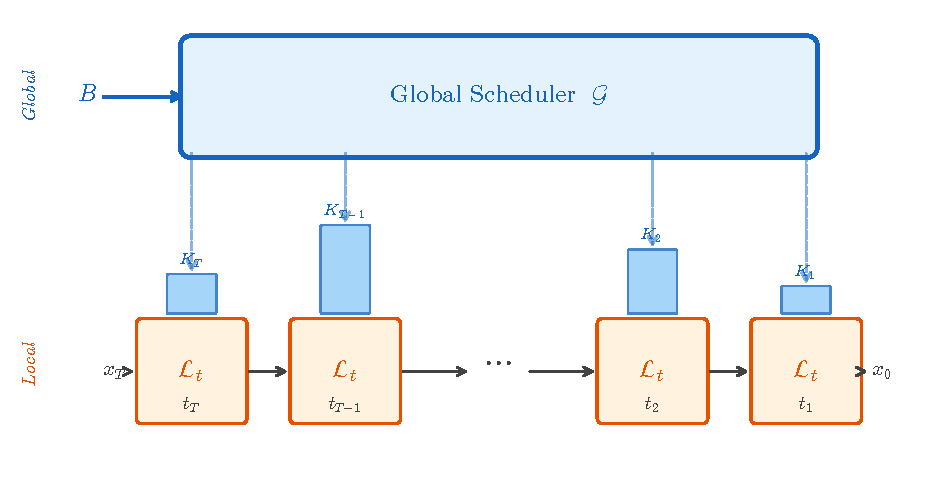
\includegraphics[width=\linewidth]{figures/fig_architecture.pdf}
\caption{Two-level view of noise trajectory search.
The \emph{global scheduler}~$\mathcal{G}$ (top) takes a total budget~$B$
and distributes per-step budgets $\{K_t\}$ across the denoising trajectory.
At each timestep, a \emph{local search operator}~$\mathcal{L}_t$ (bottom)
evaluates $K_t$ noise candidates and selects the best one.
The bars above each step visualize the non-uniform allocation:
timesteps where noise perturbations matter more receive larger budgets.}
\label{fig:architecture}
\end{figure}

\paragraph{Local search operator.}
At a single timestep $t$, given a current latent $x_t$, conditioning $c$,
verifier $v$, and base sampler $F_\theta$, a \emph{local} search operator
\[
  \mathcal{L}_t : (x_t, c, v, F_\theta, \text{budget at } t)
  \longrightarrow (x_{t-1}, \varepsilon_t)
\]
tries multiple noise candidates $\varepsilon_t$ and selects the one that
yields the highest verifier score.
To evaluate a candidate noise $\varepsilon_t^{(k)}$, we first apply the
base sampler to obtain the next-step latent and its associated clean-output
prediction in a single network evaluation:
\begin{equation}
  x_{t-1}^{(k)} = F_\theta(x_t,\, t,\, c,\, \varepsilon_t^{(k)}),
  \qquad
  \hat{x}_0^{(k)} = D_\theta(x_{t-1}^{(k)},\, t\!-\!1,\, c),
  \label{eq:x0_prediction}
\end{equation}
where $D_\theta$ denotes the model's denoising prediction (Tweedie's
estimate~\citep{song2021scorebased}), an intermediate output of the
denoising network that maps any noisy latent to a clean-output estimate.
The verifier then scores this prediction:
\begin{equation}
  s^{(k)} = v\!\bigl(\hat{x}_0^{(k)},\, c\bigr).
  \label{eq:score}
\end{equation}
In a single local search iteration, $K$ candidate noises
$\{\varepsilon_t^{(k)}\}_{k=1}^K$ are sampled, scored via
\cref{eq:x0_prediction,eq:score}, and the best candidate
$k^* = \arg\max_k s^{(k)}$ is selected.
Each candidate evaluation costs one function evaluation (one forward pass
through the denoising network), so $K$ candidates consume $K$ NFE.
Many existing noise search procedures---zero-order perturbation,
$\epsilon$-greedy exploration, particle-based
refinement---are specific instantiations of this operator; here we treat
$\mathcal{L}_t$ abstractly as a black-box mapping from $x_t$ to $x_{t-1}$
given a per-step budget.

\paragraph{Global scheduler over timesteps.}
While the local operator $\mathcal{L}_t$ decides \emph{how} to search at a given
step once we commit to spend budget there, it does not specify \emph{where
along the denoising trajectory} we should invest computation.
A global scheduler is then
\[
  \mathcal{G} :
  \bigl(x_T, c, v, F_\theta, B, \{\mathcal{L}_t\}_{t=1}^T\bigr)
  \longrightarrow \bigl(x_0, \{x_t\}_{t=1}^T\bigr),
\]
which, starting from an initial noise $x_T \sim \mathcal{N}(0, I)$, repeatedly
applies denoising steps and local search under a total compute budget $B$ and
returns both the final sample $x_0$ and the whole latent trajectory
$\{x_t\}_{t=1}^T$.

Operationally, the scheduler $\mathcal{G}$ traverses timesteps from $T$ to $1$.
At each step $t$ it decides whether to:
(i) invoke the local operator $\mathcal{L}_t$ one or multiple times, consuming
part of the remaining budget at this timestep, or
(ii) skip local search and directly apply a single base sampler step
$x_{t-1} = F_\theta(x_t, t, c, \varepsilon_t)$.
The key challenge is that this decision must be made \emph{online}: at step $t$
we do not yet know how effective search will be at later timesteps, but any
computation used now cannot be reused later.
Our goal is to design global scheduling policies that decide, under a fixed NFE
budget, \emph{on which timesteps to search and for how long}.

This two-level view --- a local operator $\mathcal{L}_t$ and a global scheduler
$\mathcal{G}$ --- provides a common language that covers many prior
inference-time search strategies:
\begin{itemize}
  \item \textbf{Plain diffusion sampling.}
  If we let $\mathcal{L}_t$ be a single base denoising step and never allocate
  extra budget, the scheduler $\mathcal{G}$ simply applies $F_\theta$ once per
  timestep, recovering the standard sampler without search.
  \item \textbf{Best-of-$N$ / random search.}
  Taking multiple i.i.d.\ initial noises, propagating each to time $0$ without
  modifying noises, and finally selecting the best $x_0$ corresponds to a
  scheduler that invests all compute into running full trajectories and only
  performs a global selection at the end; there is effectively no local search.
  \item \textbf{Noise-trajectory and tree-style search.}
  Methods that iteratively refine a noise pivot or expand/prune partial
  trajectories at certain timesteps can be interpreted as choosing specific
  forms of $\mathcal{L}_t$ and hard-coded policies in $\mathcal{G}$ that decide
  on which timesteps to apply search and how to split budget across time.
\end{itemize}
In the remainder of this section we focus on a particular and practically
important family of methods and develop a new global scheduler within this
framework.
